\documentclass{beamer}

\usetheme{Berkeley}

\usepackage{hyperref}
%\usepackage{mve}

\title{The purpose of existence \\ A question easily answered in 20 minutes}
\author{Niels Lachat, 3MG01 \\ $\varphi$}
\date{March 2018}

\AtBeginSection[]
{
  \begin{frame}
    \frametitle{Table of Contents}
    \tableofcontents[currentsection]
  \end{frame}
}

\begin{document}

	\maketitle
	
	\tableofcontents
	
	\section{Definition of the question}
	
	\begin{frame}
		\frametitle{A little introduction} 
		\href{../orig.gif}{For a better understanding of the question...} \pause
		
		%Why is it worth doing what we do every day? What is the *greater good* for which we all live? Is there any "great purpose" for which we all live? I question the purpose of each and every thing that exists.
		\begin{itemize}[<+->]
			\item What is the purpose of existence?
			\item What is the finality of everything? 
		\end{itemize}
		\pause
		%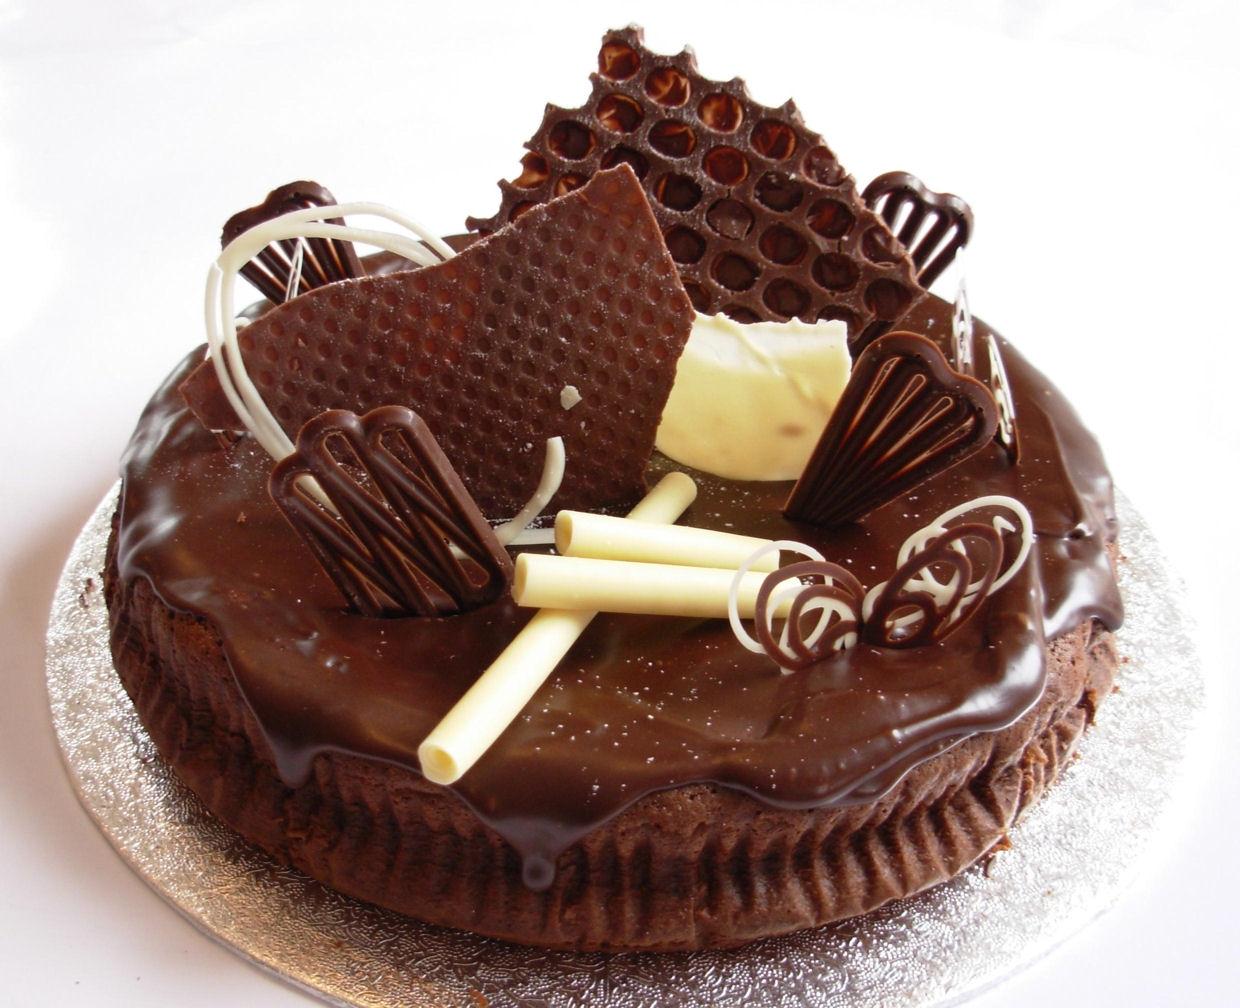
\includegraphics[scale=.1]{../cake}
		
		
		\begin{center}
		\begin{tabular}{lll}
			\raisebox{-.5\height}{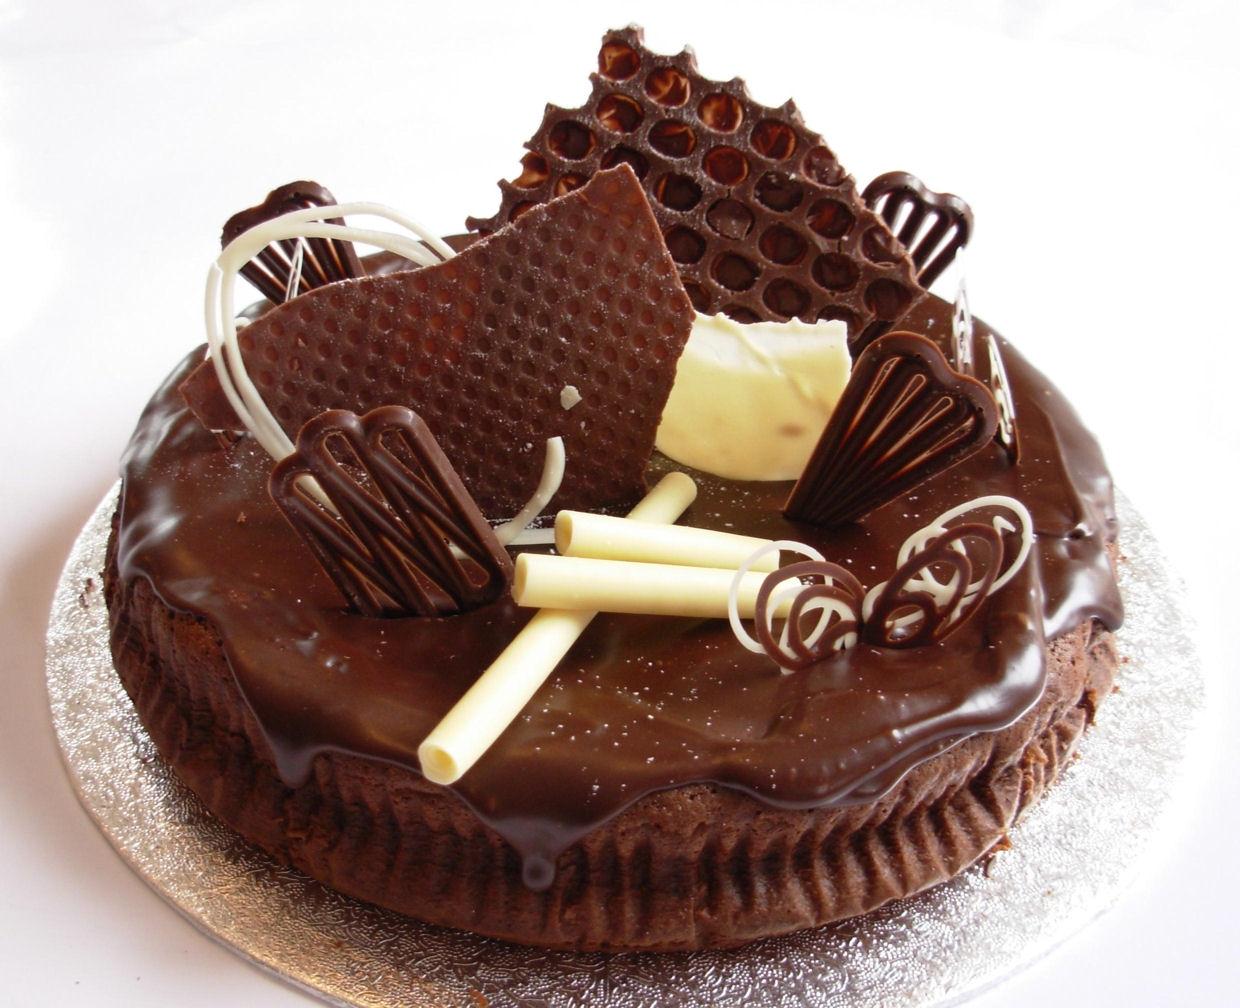
\includegraphics[scale=0.1]{../cake}} & \Huge{$\Rightarrow$} & \Huge{?}\\
		\end{tabular}
		\end{center}
    \end{frame}
    
    
    \section{Why this question?}
    \begin{frame}
    		\frametitle{The origin of my questionning}
    		
    		\begin{itemize}[<+->]
    			\item A stressful period
    			\item $\Rightarrow$ Why even bother? 
    			\item What is it all about?
    		\end{itemize}
    \end{frame}
    
    
    \section{The first answers}
    
    \begin{frame}
    	\frametitle{The answers are simple \footnote{Or are they?}}
    	
		To the question: "Why even bother?" \pause    		
		\begin{itemize}[<+->]
			\item Why study? $\Rightarrow$ To get a good job.
			\item Why get a good job? $\Rightarrow$ To have enough money.
			\item Why have enough money? $\Rightarrow$ To survive.
			\item \textbf{Why survive?}
		\end{itemize}		    		
    \end{frame}
    
	\section{The greater goals}    
    
    \begin{frame}
    		\frametitle{Advancement of science!}
    		
    		The greatest of all goals!\footnote{Or is it?} \pause
    		\begin{itemize}[<+->]
    			\item Profits to the rich
    			\item Some terrible discoveries (atom bombs, mass control, \dots)
    			\item \textbf{What's the aim?}
    		\end{itemize}
    \end{frame}
    
    \begin{frame}
    	\frametitle{Ecology}
    		
    	Ecology! \pause
    	\begin{itemize}[<+->]
    		\item Survival of the human species 
    		\item Survival of life on earth
    	\end{itemize}
    		
	\pause
    	\textbf{But what does it change?} At the end $\Rightarrow$ Big Crunch or Infinite expansion (endless cooldown $\Rightarrow$ death of all life)
    		
    		
    	%Is life very different from non-life? (soul: not proven to exist, spirit? neither)
    \end{frame}
    
    \section{New answers} %plural ?    
    \begin{frame}
    	\frametitle{Nina's answer}
    		
    	\textit{"What if the aim of life is to answer your questionnings?" \\
    \begin{flushright}
    	Nina Ionescu, 16.02.2018
    \end{flushright}}
    	%not satisfactory: What if there is no answer? I'll have spent my life looking for something that doesn't exist
    \end{frame}
    \begin{frame}
    	\frametitle{Voltaire's Answers in \textit{Candide}}
    	
    	\begin{center}
    	\textit{"Travaillons sans raisonner, c'est le seul moyen de rendre la vie supportable."} \\ \pause
    	or \\ \pause
    	\textit{"Cela est bien, dit Candide, mais il faut cultiver notre jardin."}
    	\end{center}	
    	%Acceptable answers, but still frustrating
    \end{frame}
    
    \section{The best worst answer}
    
    \begin{frame}
    	\frametitle{There is no purpose}
    	%Maybe the most satisfactory answer. Nothing has any importance.
    	There is no answer. \\ \pause
    	Everything exists only by pure randomness. \\ \pause
    	\begin{alertblock}{Consequence}
    		$\Rightarrow$ \textbf{Calls every aspect of our lives into question.}
		\end{alertblock}
    \end{frame}
    
    %\section{Resulting paradoxes} maybe...
    
    \section{Discussion}
    
    \begin{frame}
    	\frametitle{Discussion}
    	
    	\begin{center}
    	Maybe I just don't have the answer, but somebody else has. \\
    	What would your answer be?
    	\end{center}
    	
    \end{frame}
    
\end{document}